\documentclass[11pt,oneside,openany]{book}

% ============================================================
% Versatus HPC Book Template v0.2.3 — Dynamic Cover Test Harness
% Engine  : LuaLaTeX
% Purpose : Isolated test file for the automation pipeline.
%           Compiles the dynamic cover without touching main.tex.
%
% To generate and compile:
%   python automation/scripts/build_cover.py <cover_image.png>
%
% To recompile with an existing canvas JSON (skip Vision API):
%   python automation/scripts/build_cover.py --skip-vision
% ============================================================

% ============================================================
% Document metadata
% Edit this file for each book project.
% ============================================================

\newcommand{\BookTitle}{Título do Livro Técnico}
\newcommand{\BookSubtitle}{Subtítulo científico ou programa de estudos}
\newcommand{\BookDescription}{Material técnico de formação, referência e estudo}
\newcommand{\BookAuthor}{Autor / Organização}
\newcommand{\BookDate}{\today}
\newcommand{\BookVersion}{v0.1}
\newcommand{\BookConfidentiality}{Uso interno / rascunho técnico}
\newcommand{\BookSeries}{Série Técnica}

% Default variant and cover if the user compiles main.tex directly.
\providecommand{\VSDocumentVariant}{standard}
\providecommand{\VSCoverOption}{A}

\usepackage{styles/versatus-colors}
\usepackage{styles/versatus-variant}
\usepackage{styles/versatus-typography}
\usepackage{styles/versatus-layout}
\usepackage{styles/versatus-environments}
\usepackage{styles/versatus-covers}

% ── Dynamic cover macro ───────────────────────────────────────────────────────
% This file is generated by automation/scripts/build_cover.py.
% If it does not exist yet (first run before the pipeline), a placeholder
% is rendered so this document compiles cleanly regardless.
\IfFileExists{styles/versatus-dynamic-cover.tex}{%
  % Auto-generated by vision_extractor.py (brand: kosen) - DO NOT EDIT MANUALLY
% === Brand preamble: Kosen Energy ===
\IfFontExistsTF{Work Sans}{
  \setmainfont{Work Sans}\setsansfont{Work Sans}%
}{\IfFontExistsTF{Noto Sans}{
  \setmainfont{Noto Sans}\setsansfont{Noto Sans}%
}{\setmainfont{Latin Modern Sans}\setsansfont{Latin Modern Sans}}}
\definecolor{VSBlack}{HTML}{4038FF}
\definecolor{VSGraphite}{HTML}{C7B99C}
\definecolor{VSTeal}{HTML}{C7B99C}
\definecolor{VSRed}{HTML}{757576}
\definecolor{VSSilver}{HTML}{C6C6C8}
\definecolor{VSPaperWhite}{HTML}{FFFFFF}
\definecolor{VSMutedText}{HTML}{757576}
\definecolor{VSCoverFg}{HTML}{1A1A1A}
\definecolor{VSCoverSubFg}{HTML}{757576}
\definecolor{VSCoverMutedFg}{HTML}{757576}
\definecolor{VSCoverFaintFg}{HTML}{757576}
\renewcommand{\BookSeries}{Kosen Energy Technical Books}
% === end brand preamble ===
% Auto-generated from logo_dark.svg by svg_to_tikz.py - DO NOT EDIT MANUALLY
\newcommand{\LogoKosenDark}[1]{%
    \begingroup
    \definecolor{LogoKosenDarkC0}{HTML}{4038FF}
    \definecolor{LogoKosenDarkC1}{HTML}{C6C6C8}
    \begin{scope}[shift={#1}]
        \fill[LogoKosenDarkC0] (6.28,1.217) rectangle (6.563,1.5);
        \fill[LogoKosenDarkC1] (1.015,0) -- (0.491,0.68) -- (1.009,1.217) -- (0.841,1.217) -- (0.146,0.529) -- (0.118,0.529) -- (0.118,1.217) -- (0,1.217) -- (0,0) -- (0.118,0) -- (0.118,0.354) -- (0.406,0.604) -- (0.871,0) -- (1.015,0) -- cycle (1.315,1.396) -- (2.299,1.396) -- (2.299,1.5) -- (1.315,1.5) -- (1.315,1.396) -- cycle (2.264,0.605) .. controls (2.264,0.317) and (2.085,0.109) .. (1.806,0.109) .. controls (1.528,0.109) and (1.348,0.305) .. (1.348,0.605) .. controls (1.348,0.886) and (1.525,1.101) .. (1.806,1.101) .. controls (2.087,1.101) and (2.264,0.898) .. (2.264,0.605) (2.382,0.605) .. controls (2.382,0.957) and (2.155,1.209) .. (1.806,1.209) .. controls (1.457,1.209) and (1.23,0.957) .. (1.23,0.605) .. controls (1.23,0.253) and (1.457,0.001) .. (1.806,0.001) .. controls (2.155,0.001) and (2.382,0.253) .. (2.382,0.605) (3.579,0.864) -- (3.671,0.93) .. controls (3.548,1.103) and (3.364,1.209) .. (3.123,1.209) .. controls (2.882,1.209) and (2.701,1.093) .. (2.701,0.895) .. controls (2.701,0.697) and (2.847,0.617) .. (3.09,0.574) -- (3.227,0.551) .. controls (3.411,0.52) and (3.548,0.466) .. (3.548,0.329) .. controls (3.548,0.192) and (3.413,0.104) .. (3.22,0.104) .. controls (3.026,0.104) and (2.835,0.175) .. (2.734,0.411) -- (2.627,0.364) .. controls (2.748,0.1) and (2.977,0.001) .. (3.222,0.001) .. controls (3.468,0.001) and (3.666,0.123) .. (3.666,0.336) .. controls (3.666,0.548) and (3.482,0.619) .. (3.253,0.659) -- (3.116,0.683) .. controls (2.944,0.713) and (2.819,0.763) .. (2.819,0.9) .. controls (2.819,1.037) and (2.958,1.105) .. (3.123,1.105) .. controls (3.288,1.105) and (3.463,1.039) .. (3.579,0.864) (4.014,0.683) .. controls (4.042,0.942) and (4.222,1.1) .. (4.462,1.1) .. controls (4.703,1.1) and (4.875,0.956) .. (4.885,0.683) -- (4.014,0.683) -- cycle (4.014,0.579) -- (5.008,0.579) -- (5.008,0.654) .. controls (5.008,1.004) and (4.779,1.209) .. (4.462,1.209) .. controls (4.146,1.209) and (3.891,0.952) .. (3.891,0.614) .. controls (3.891,0.277) and (4.123,0.001) .. (4.479,0.001) .. controls (4.783,0.001) and (4.913,0.168) .. (4.991,0.329) -- (4.878,0.374) .. controls (4.812,0.225) and (4.701,0.109) .. (4.479,0.109) .. controls (4.212,0.109) and (4.031,0.286) .. (4.014,0.579) (6.275,0.034) -- (6.275,0.732) .. controls (6.275,1.051) and (6.058,1.2) .. (5.817,1.2) .. controls (5.577,1.2) and (5.456,1.079) .. (5.393,0.959) -- (5.36,0.959) -- (5.36,1.176) -- (5.246,1.176) -- (5.246,0.034) -- (5.364,0.034) -- (5.364,0.605) .. controls (5.364,0.931) and (5.551,1.091) .. (5.794,1.091) .. controls (6.013,1.091) and (6.157,0.983) .. (6.157,0.723) -- (6.157,0.034) -- (6.275,0.034) -- cycle;
    \end{scope}
    \endgroup
}
% Auto-generated from logo_simbol.svg by svg_to_tikz.py - DO NOT EDIT MANUALLY
\newcommand{\LogoKosenAlt}[1]{%
    \begingroup
    \definecolor{LogoKosenAltC0}{HTML}{4038FF}
    \definecolor{LogoKosenAltC1}{HTML}{E5E5E5}
    \begin{scope}[shift={#1}]
        \fill[LogoKosenAltC0] (0,0) rectangle (1.514,1.5);
        \fill[LogoKosenAltC1] (1.214,1.244) -- (1.079,1.244) -- (0.519,0.69) -- (0.497,0.69) -- (0.497,1.244) -- (0.402,1.244) -- (0.402,0.265) -- (0.497,0.265) -- (0.497,0.55) -- (0.728,0.751) -- (1.103,0.265) -- (1.218,0.265) -- (0.797,0.812) -- (1.214,1.244) -- cycle;
    \end{scope}
    \endgroup
}
\renewcommand{\VSBrandFooterLogo}{%
  \resizebox{!}{0.50cm}{%
    \begin{tikzpicture}[baseline=(current bounding box.south)]%
      \LogoKosenAlt{(0,0)}%
    \end{tikzpicture}%
  }%
}
\renewcommand{\VSBrandWatermark}{%
  \ifVSWatermark
  \begin{tikzpicture}[remember picture, overlay]%
    \node[opacity=0.030, anchor=center, inner sep=0pt]
      at (current page.center)
      {\resizebox{12cm}{!}{%
        \begin{tikzpicture}%
          \LogoKosenDark{(0,0)}%
        \end{tikzpicture}%
      }};
  \end{tikzpicture}%
  \fi
}
\newcommand{\RenderDynamicCover}{%
% LOGO_PLACEMENT x=1.0 y=27.0 height=1.5 bg=bg_primary
\definecolor{bg_primary}{HTML}{4038FF}
\definecolor{bg_secondary}{HTML}{C7B99C}
\definecolor{accent_1}{HTML}{C7B99C}
\definecolor{accent_2}{HTML}{3B3CD0}
\definecolor{neutral}{HTML}{C6C6C8}
\definecolor{light}{HTML}{FFFFFF}
\definecolor{muted}{HTML}{757576}
\begin{tikzpicture}[remember picture, overlay,
  shift={(current page.south west)}, x=1cm, y=1cm]
  %
  % --- BACKGROUND ---
  %
  % Footer area
  \fill[light] (-1,-1) rectangle (22, 8.5);
  
  % Bottom row of geometric blocks
  \fill[accent_2] (-1, 8.5) rectangle (15.75, 14.5);
  \fill[muted] (15.75, 8.5) rectangle (22, 14.5);
  
  % Middle row of geometric blocks
  \fill[bg_primary] (-1, 14.5) rectangle (5.25, 23.5);
  % Middle-center split square
  \fill[neutral] (5.25, 14.5) -- (5.25, 23.5) -- (15.75, 23.5) -- cycle;
  \fill[accent_1] (5.25, 14.5) -- (15.75, 14.5) -- (15.75, 23.5) -- cycle;
  \fill[bg_secondary] (15.75, 14.5) rectangle (22, 23.5);
  
  % Top row of geometric blocks
  \fill[bg_primary] (-1, 23.5) rectangle (5.25, 30.7);
  \fill[accent_2] (5.25, 23.5) rectangle (15.75, 30.7);
  \fill[bg_secondary] (15.75, 23.5) rectangle (22, 30.7);
  
  % --- TEXT ---
  %
  % Main Title
  \node[anchor=north west, text width=19cm, align=flush left] at (0.8, 8.2) {%
    {\fontsize{54}{60}\selectfont\bfseries\color{VSCoverFg}\BookTitle}%
  };
  
  % Separator Line
  \draw[VSRed, line width=1.2pt] (0.8, 3.2) -- (20.2, 3.2);
  
  % Three-column footer text
  \node[anchor=south west, text width=6cm, align=flush left] at (0.8, 1.2) {%
    {\fontsize{10}{12}\selectfont\color{VSCoverSubFg}\BookSubtitle}%
  };
  
  \node[anchor=south west, text width=6cm, align=flush left] at (7.5, 1.2) {%
    {\fontsize{10}{12}\selectfont\color{VSCoverSubFg}\BookDescription}%
  };
  
  \node[anchor=south west, text width=5.5cm, align=flush left] at (14.5, 1.2) {%
    {\fontsize{10}{12}\selectfont\color{VSCoverMutedFg}\BookAuthor}\\[0.1cm]
    {\fontsize{9}{11}\selectfont\color{VSCoverFaintFg}\BookDate\ |\ \BookVersion}%
  };
  
  \LogoKosenDark{(1.0, 27.0)}
\end{tikzpicture}%
}
%
}{%
  \newcommand{\RenderDynamicCover}{%
    \begin{tikzpicture}[remember picture, overlay]
      \fill[black!12]
        (current page.south west) rectangle (current page.north east);
      \node[
        font=\Large\sffamily,
        text=black!45,
        align=center,
        text width=12cm
      ] at (current page.center) {%
        Dynamic cover not generated yet.\\[8pt]
        \normalsize\ttfamily
        python automation/scripts/build\_cover.py <image.png>%
      };
    \end{tikzpicture}%
  }%
}

\hypersetup{
  pdftitle={\BookTitle},
  pdfauthor={\BookAuthor},
  pdfsubject={\BookSubtitle},
  pdfkeywords={Versatus HPC, dynamic cover, automation pipeline}
}

\begin{document}

% ── Dynamic cover page ────────────────────────────────────────────────────────
% \VSBookCoverDynamic = \RenderDynamicCover (VLM geometry) + text overlay
% from config/metadata.tex (\BookTitle, \BookSubtitle, \BookAuthor, etc.).
\VSBookCoverDynamic

% ── Document body (uncomment to compile the full document) ────────────────────
%
% \frontmatter
% \input{frontmatter/toc}
%
% \mainmatter
% \chapter{Estruturas de Texto e Tabelas}

Este capítulo funciona como uma página de referência para o desenho interno de livros técnicos da Versatus HPC. O conteúdo é propositalmente genérico: ele deve ser substituído pelo texto real do projeto, mas preserva exemplos de hierarquia, ritmo editorial, tabelas e parágrafos contínuos. A intenção é facilitar a validação do template antes do início da escrita final.

\section{Três parágrafos contínuos}

A documentação técnica deve privilegiar uma sequência de leitura estável: contexto, decisão, justificativa e consequência. Em materiais didáticos, essa ordem reduz ambiguidade e evita que o leitor precise inferir a arquitetura mental do autor. O texto corrido deve ser usado quando a explicação depende de continuidade conceitual, especialmente em capítulos introdutórios, fundamentos teóricos e discussões de projeto.

Em documentos de engenharia, parágrafos longos demais tendem a prejudicar a manutenção editorial. A recomendação é preservar blocos com uma ideia central por parágrafo, usando listas apenas quando houver enumeração real. Essa disciplina ajuda a converter o mesmo conteúdo em livro, manual, relatório técnico ou white paper sem reescrita estrutural excessiva.

Para programas de estudo, a redação deve separar claramente conceitos estáveis, hipóteses de trabalho, exemplos, restrições e decisões normativas. Essa separação permite que o material seja usado tanto para leitura sequencial quanto para consulta posterior. O template foi desenhado para aceitar ambos os modos sem alterar a identidade visual.

\section{Tabela pequena}

A tabela pequena deve ser usada para parâmetros, convenções, nomenclaturas ou comparações curtas. Ela não deve dominar a página.

\begin{table}[htbp]
\centering
\caption{Exemplo de tabela pequena}
\label{tab:pequena}
\begin{tabular}{lll}
\toprule
Item & Valor & Observação \\
\midrule
CPU & 2 sockets & Nós de computação \\
GPU & 8 unidades & Treinamento de modelos \\
Rede & 400 Gb/s & Interconexão de baixa latência \\
\bottomrule
\end{tabular}
\end{table}

\section{Tabela média}

A tabela média é indicada quando há mais texto por célula. Neste caso, \texttt{tabularx} permite que as colunas se ajustem à largura útil da página.

\begin{table}[htbp]
\centering
\caption{Exemplo de tabela média com largura controlada}
\label{tab:media}
\begin{tabularx}{\textwidth}{>{\bfseries}p{0.22\textwidth}X X}
\toprule
Categoria & Uso recomendado & Critério de aceite \\
\midrule
Provisionamento & Descrever instalação, imagem base, dependências e sequência de boot. & O leitor consegue reproduzir o ambiente sem decisões implícitas. \\
Operação & Explicar rotinas administrativas, telemetria e tratamento de falhas. & O procedimento apresenta pré-condições, passos e rollback. \\
Validação & Registrar testes, métricas, hipóteses e limites conhecidos. & Os resultados são rastreáveis e repetíveis. \\
\bottomrule
\end{tabularx}
\end{table}

\section{Tabela grande}

A tabela grande deve ser usada com moderação. Em livros e manuais, ela é útil para matrizes de requisitos, listas de componentes, parâmetros de configuração e inventários técnicos. Quando a tabela atravessar páginas, use \texttt{longtable}.

{\scriptsize
\setlength{\tabcolsep}{3pt}
\begin{longtable}{p{0.08\textwidth}p{0.15\textwidth}p{0.14\textwidth}p{0.12\textwidth}p{0.16\textwidth}p{0.14\textwidth}p{0.11\textwidth}}
\caption{Exemplo de tabela grande com múltiplas linhas}\label{tab:grande}\\
\toprule
ID & Componente & Função & Prioridade & Métrica & Evidência & Estado \\
\midrule
\endfirsthead
\toprule
ID & Componente & Função & Prioridade & Métrica & Evidência & Estado \\
\midrule
\endhead
\midrule
\multicolumn{7}{r}{Continua na próxima página}\\
\endfoot
\bottomrule
\endlastfoot
R01 & Kernel & Base de execução do sistema & Alta & Latência e estabilidade & Testes de carga & Aberto \\
R02 & Rede & Comunicação entre nós & Alta & Vazão e perda de pacotes & Benchmarks sintéticos & Aberto \\
R03 & Storage & Persistência paralela & Alta & IOPS e throughput & IOR, mdtest & Aberto \\
R04 & Scheduler & Alocação de recursos & Alta & Tempo de fila & Simulações de workload & Aberto \\
R05 & Observabilidade & Eventos e métricas & Média & Custo de coleta & Telemetria contínua & Aberto \\
R06 & Segurança & Controle de acesso & Alta & Superfície exposta & Revisão de configuração & Aberto \\
R07 & Documentação & Reprodutibilidade & Média & Cobertura editorial & Checklist de publicação & Aberto \\
R08 & CI/CD & Geração de artefatos & Média & Tempo de build & Pipeline automatizado & Aberto \\
R09 & Instalação & Primeira implantação & Alta & Taxa de sucesso & Testes em ambiente limpo & Aberto \\
R10 & Atualização & Evolução controlada & Média & Rollback funcional & Ensaios de versão & Aberto \\
R11 & Diagnóstico & Suporte operacional & Média & Tempo de triagem & Casos simulados & Aberto \\
R12 & Treinamento & Transferência de conhecimento & Baixa & Conclusão dos módulos & Avaliação interna & Aberto \\
\end{longtable}
}

% \chapter{Equações e Modelos Matemáticos}

Este capítulo apresenta exemplos de equações pequenas, médias e grandes. A finalidade é validar espaçamento, numeração, quebras de linha, referências cruzadas e integração visual entre texto técnico e formalismo matemático.

\section{Equação pequena}

Equações pequenas podem aparecer em linha, como $E = mc^2$, ou em modo destacado quando forem usadas como referência posterior:

\begin{equation}
\label{eq:pequena}
T = \frac{D}{B}.
\end{equation}

Na \cref{eq:pequena}, $T$ representa tempo, $D$ representa volume de dados e $B$ representa largura de banda efetiva.

\section{Equação média}

Equações médias costumam ocupar quase uma linha inteira. Elas devem permanecer legíveis, sem compressão manual excessiva.

\begin{equation}
\label{eq:media}
\mathcal{C}_{\mathrm{total}}(n,m,k)=\alpha n + \beta m\log_2(m) + \gamma k^2 + \delta\sum_{i=1}^{n}\frac{x_i}{1+\rho_i}.
\end{equation}

A \cref{eq:media} ilustra uma expressão composta por termos lineares, logarítmicos, quadráticos e uma soma ponderada. Em documentação técnica, esse formato é adequado para modelos de custo, estimativas de capacidade e hipóteses analíticas.

\section{Equação grande em múltiplas linhas}

Equações grandes devem usar ambientes como \texttt{align}, \texttt{aligned} ou \texttt{multline}. O objetivo é preservar alinhamento sem sacrificar leitura.

\begin{align}
\label{eq:grande}
\mathcal{L}(\theta) &=
\sum_{b=1}^{B}\left[
  \frac{1}{N_b}\sum_{i=1}^{N_b}
  \left\| f_{\theta}(x_{b,i}) - y_{b,i} \right\|_2^2
\right]
+ \lambda_1\left\|\theta\right\|_1
+ \lambda_2\left\|\theta\right\|_2^2 \\
&\quad + \eta\sum_{j=1}^{J}
\max\left(0,\tau_j - q_j(\theta)\right)^2
+ \mu\sum_{r=1}^{R}
\left| c_r(\theta)-\widehat{c}_r \right|.
\end{align}

A \cref{eq:grande} mostra uma função objetivo com termo empírico, regularização, penalidades de restrição e distância a metas operacionais. Esse tipo de bloco é comum em capítulos de otimização, modelagem de desempenho e aprendizado de máquina.

\section{Bloco técnico com equação}

\begin{VSNote}[title={Regra editorial para matemática}]
Use equações numeradas quando elas forem citadas, discutidas ou reutilizadas. Use equações não numeradas apenas para derivações locais ou exemplos transitórios. Evite transformar texto explicativo em sequência de símbolos quando o argumento puder ser expresso de forma mais clara em linguagem natural.
\end{VSNote}

% \chapter{Figuras, Gráficos e Blocos Multicoluna}

Este capítulo reúne exemplos visuais usados com frequência em materiais técnicos: gráficos individuais, painéis de gráficos, fotografia centralizada, fotografia acompanhada de texto e blocos editoriais em duas, três e quatro colunas.

\ifVSColor
  \def\VSPlotAColor{VSRed}
  \def\VSPlotBColor{VSTeal}
  \def\VSPlotCColor{VSBlack}
  \def\VSPlotDColor{VSSilver}
\else
  \def\VSPlotAColor{VSBlack}
  \def\VSPlotBColor{VSMutedText}
  \def\VSPlotCColor{VSBlack}
  \def\VSPlotDColor{VSSilver}
\fi

\section{Um gráfico}

\begin{figure}[H]
\centering
\begin{tikzpicture}
\begin{axis}[
  width=0.76\textwidth,
  height=6.0cm,
  grid=both,
  xlabel={Tamanho do problema},
  ylabel={Throughput normalizado},
  ymin=0,
  legend pos=south east]
\addplot+[mark=*,color=\VSPlotAColor,line width=0.9pt] coordinates {(1,1.0) (2,1.8) (4,3.2) (8,5.9) (16,9.8)};
\addlegendentry{Configuração A}
\addplot+[mark=square*,color=\VSPlotBColor,line width=0.9pt] coordinates {(1,0.8) (2,1.5) (4,2.9) (8,5.2) (16,8.7)};
\addlegendentry{Configuração B}
\end{axis}
\end{tikzpicture}
\caption{Exemplo de gráfico individual gerado em TikZ/PGFPlots}
\label{fig:grafico-unico}
\end{figure}

\section{Dois gráficos lado a lado}

\begin{figure}[H]
\centering
\begin{subfigure}[t]{0.48\textwidth}
\centering
\begin{tikzpicture}
\begin{axis}[width=\textwidth,height=5.2cm,grid=major,xlabel={Tempo},ylabel={Uso de CPU},ymin=0,ymax=100]
\addplot+[mark=none,color=\VSPlotAColor,line width=0.9pt] coordinates {(0,20) (1,28) (2,35) (3,50) (4,61) (5,66) (6,70)};
\end{axis}
\end{tikzpicture}
\caption{Série temporal}
\end{subfigure}\hfill
\begin{subfigure}[t]{0.48\textwidth}
\centering
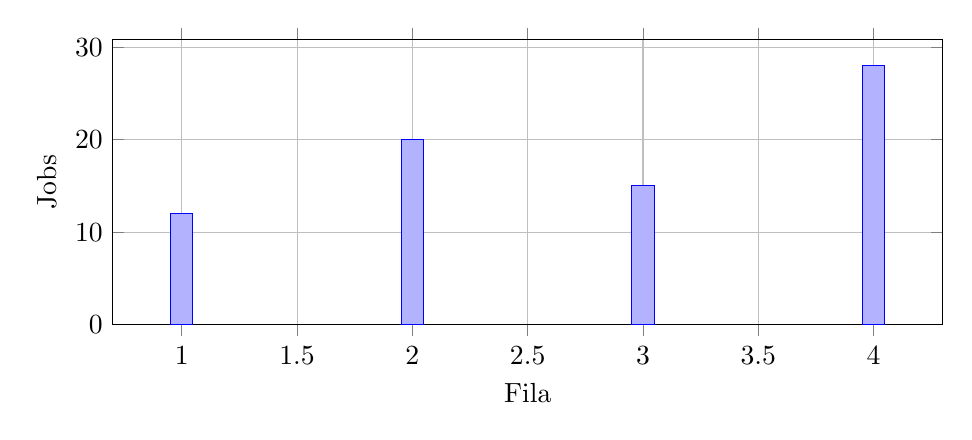
\begin{tikzpicture}
\begin{axis}[width=\textwidth,height=5.2cm,grid=major,xlabel={Fila},ylabel={Jobs},ybar,bar width=8pt,ymin=0]
\addplot+[fill=\VSPlotBColor,draw=\VSPlotBColor] coordinates {(1,12) (2,20) (3,15) (4,28)};
\end{axis}
\end{tikzpicture}
\caption{Distribuição discreta}
\end{subfigure}
\caption{Exemplo de dois gráficos lado a lado}
\label{fig:dois-graficos}
\end{figure}

\section{Quatro gráficos em matriz 2 x 2}

\begin{figure}[H]
\centering
\begin{subfigure}[t]{0.48\textwidth}
\centering
\begin{tikzpicture}
\begin{axis}[width=\textwidth,height=4.7cm,grid=major,xlabel={Amostra},ylabel={Latência}]
\addplot+[mark=*,color=\VSPlotAColor,line width=0.8pt] coordinates {(1,7) (2,6) (3,6.5) (4,5.8) (5,5.2)};
\end{axis}
\end{tikzpicture}
\caption{Latência}
\end{subfigure}\hfill
\begin{subfigure}[t]{0.48\textwidth}
\centering
\begin{tikzpicture}
\begin{axis}[width=\textwidth,height=4.7cm,grid=major,xlabel={Amostra},ylabel={IOPS}]
\addplot+[mark=square*,color=\VSPlotBColor,line width=0.8pt] coordinates {(1,10) (2,14) (3,18) (4,21) (5,25)};
\end{axis}
\end{tikzpicture}
\caption{IOPS}
\end{subfigure}

\vspace{0.4cm}

\begin{subfigure}[t]{0.48\textwidth}
\centering
\begin{tikzpicture}
\begin{axis}[width=\textwidth,height=4.7cm,grid=major,xlabel={Amostra},ylabel={Eficiência},ymin=0,ymax=1]
\addplot+[mark=triangle*,color=\VSPlotCColor,line width=0.8pt] coordinates {(1,0.60) (2,0.66) (3,0.71) (4,0.75) (5,0.78)};
\end{axis}
\end{tikzpicture}
\caption{Eficiência}
\end{subfigure}\hfill
\begin{subfigure}[t]{0.48\textwidth}
\centering
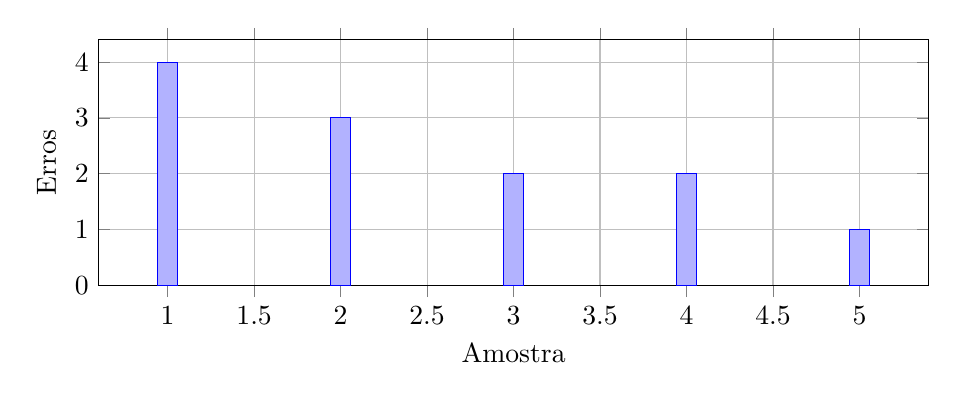
\begin{tikzpicture}
\begin{axis}[width=\textwidth,height=4.7cm,grid=major,xlabel={Amostra},ylabel={Erros},ybar,bar width=7pt,ymin=0]
\addplot+[fill=\VSPlotDColor,draw=\VSPlotCColor] coordinates {(1,4) (2,3) (3,2) (4,2) (5,1)};
\end{axis}
\end{tikzpicture}
\caption{Erros}
\end{subfigure}
\caption{Exemplo de quatro gráficos organizados em duas linhas e duas colunas}
\label{fig:quatro-graficos}
\end{figure}

\section{Foto centralizada}

\begin{figure}[H]
\centering

\includegraphics[width=0.82\textwidth]{assets/figures/versatus-photo-placeholder.png}
\caption{Exemplo de fotografia centralizada. Substitua o arquivo por uma fotografia real do produto, laboratório, cluster ou instalação.}
\label{fig:foto-centralizada}
\end{figure}

\section{Foto com texto ao lado}

\begin{figure}[H]
\centering
\begin{minipage}[c]{0.47\textwidth}

\includegraphics[width=\textwidth]{assets/figures/versatus-photo-placeholder.png}
\end{minipage}\hfill
\begin{minipage}[c]{0.48\textwidth}
\textbf{Uso recomendado.} Esta composição é adequada para explicar uma imagem sem deslocar o leitor para outra página. Ela funciona bem em manuais, livros de laboratório, lâminas técnicas e relatórios de validação.

\textbf{Critério editorial.} O texto lateral deve interpretar a imagem, não repetir a legenda. Para fotografias de produto, descreva o contexto, o componente visível, o papel operacional e a evidência técnica.
\end{minipage}
\caption{Exemplo de fotografia acompanhada de texto lateral}
\label{fig:foto-texto-lado}
\end{figure}

\section{Dois blocos em duas colunas}

\noindent\begin{minipage}[t]{0.48\textwidth}
\begin{VSNote}[title={Bloco 1}]
Use duas colunas quando houver comparação direta entre conceitos, decisões arquiteturais, variantes de produto ou modos de operação.
\end{VSNote}
\end{minipage}\hfill
\begin{minipage}[t]{0.48\textwidth}
\begin{VSNote}[title={Bloco 2}]
Evite colunas longas demais. Se o conteúdo exigir mais de meia página, prefira uma seção convencional com subtítulos.
\end{VSNote}
\end{minipage}

\section{Três blocos em três colunas}

\noindent\begin{minipage}[t]{0.31\textwidth}
\begin{VSProcedure}[title={Entrada}]
Defina pré-condições, arquivos, parâmetros e dependências externas.
\end{VSProcedure}
\end{minipage}\hfill
\begin{minipage}[t]{0.31\textwidth}
\begin{VSProcedure}[title={Processo}]
Liste os passos principais e destaque comandos ou decisões manuais.
\end{VSProcedure}
\end{minipage}\hfill
\begin{minipage}[t]{0.31\textwidth}
\begin{VSProcedure}[title={Saída}]
Registre artefatos, logs, métricas, relatórios e critérios de aceite.
\end{VSProcedure}
\end{minipage}

\section{Quatro blocos em quatro colunas}

\noindent\begin{minipage}[t]{0.235\textwidth}
\begin{VSNote}[title={Contexto}]
\small Descreva o problema técnico.
\end{VSNote}
\end{minipage}\hfill
\begin{minipage}[t]{0.235\textwidth}
\begin{VSNote}[title={Decisão}]
\small Declare a escolha adotada.
\end{VSNote}
\end{minipage}\hfill
\begin{minipage}[t]{0.235\textwidth}
\begin{VSNote}[title={Evidência}]
\small Aponte teste, métrica ou fonte.
\end{VSNote}
\end{minipage}\hfill
\begin{minipage}[t]{0.235\textwidth}
\begin{VSNote}[title={Risco}]
\small Registre limitações e mitigação.
\end{VSNote}
\end{minipage}

% 
\chapter{Blocos de Código e Terminal}

Este capítulo apresenta exemplos de código em dois regimes editoriais: blocos escuros, adequados para simular uma sessão de terminal ou uma janela de execução, e blocos claros, adequados para leitura de código-fonte em materiais didáticos. O template usa \texttt{listings} com \texttt{tcolorbox}, evitando \texttt{minted} para preservar portabilidade sem \texttt{shell-escape}.

\section{Bloco pequeno de código em terminal}

\begin{VSTerminalCode}[title={Terminal pequeno}]
def normalize(value, scale):
    if scale == 0:
        return 0.0
    return value / scale
\end{VSTerminalCode}

\clearpage
\section{Bloco médio de código em terminal}

\begin{VSTerminalCode}[title={Terminal médio}]
def summarize_jobs(jobs):
    total_gpus = 0
    total_nodes = 0
    failed_jobs = []

    for job in jobs:
        total_gpus += job.get("gpus", 0)
        total_nodes += job.get("nodes", 0)
        if job.get("state") == "FAILED":
            failed_jobs.append(job.get("id"))

    return {
        "jobs": len(jobs),
        "gpus": total_gpus,
        "nodes": total_nodes,
        "failed": failed_jobs,
    }
\end{VSTerminalCode}

\clearpage
\section{Bloco grande de código em terminal}

\begin{VSTerminalCode}[title={Terminal grande}]
class ClusterPolicy:
    def __init__(self, max_gpus_per_user, reserved_nodes):
        self.max_gpus_per_user = max_gpus_per_user
        self.reserved_nodes = set(reserved_nodes)

    def can_schedule(self, request, usage):
        user = request["user"]
        required_gpus = request.get("gpus", 0)
        candidate_nodes = request.get("nodes", [])

        if usage.get(user, 0) + required_gpus > self.max_gpus_per_user:
            return False, "gpu quota exceeded"

        for node in candidate_nodes:
            if node in self.reserved_nodes and not request.get("admin", False):
                return False, "reserved node requested"

        if not self._has_required_topology(candidate_nodes):
            return False, "topology constraint not satisfied"

        return True, "accepted"

    def _has_required_topology(self, nodes):
        if len(nodes) <= 1:
            return True
        racks = {node.split("-")[0] for node in nodes}
        return len(racks) <= 2

policy = ClusterPolicy(max_gpus_per_user=32, reserved_nodes=["rack9-node01"])
request = {
    "user": "researcher",
    "gpus": 8,
    "nodes": ["rack1-node03", "rack1-node04"],
    "admin": False,
}
usage = {"researcher": 16}
accepted, reason = policy.can_schedule(request, usage)
print(accepted, reason)
\end{VSTerminalCode}

\clearpage
\section{Bloco pequeno de código claro}

\begin{VSCodeBlock}[title={Código pequeno}]
def bandwidth(bytes_written, seconds):
    return bytes_written / seconds
\end{VSCodeBlock}

\section{Bloco médio de código claro}

\begin{VSCodeBlock}[title={Código médio}]
def moving_average(samples, window):
    if window <= 0:
        raise ValueError("window must be positive")

    result = []
    for index in range(len(samples)):
        start = max(0, index - window + 1)
        segment = samples[start:index + 1]
        result.append(sum(segment) / len(segment))

    return result
\end{VSCodeBlock}

\clearpage
\section{Bloco grande de código claro}

\begin{VSCodeBlock}[title={Código grande}]
from dataclasses import dataclass

@dataclass
class Measurement:
    timestamp: float
    node: str
    metric: str
    value: float

class TelemetryBuffer:
    def __init__(self, limit):
        self.limit = limit
        self.samples = []

    def append(self, measurement):
        self.samples.append(measurement)
        if len(self.samples) > self.limit:
            self.samples = self.samples[-self.limit:]

    def select(self, metric, node=None):
        selected = []
        for sample in self.samples:
            if sample.metric != metric:
                continue
            if node is not None and sample.node != node:
                continue
            selected.append(sample)
        return selected

    def aggregate_mean(self, metric, node=None):
        selected = self.select(metric, node=node)
        if not selected:
            return None
        return sum(sample.value for sample in selected) / len(selected)

buffer = TelemetryBuffer(limit=10000)
buffer.append(Measurement(0.0, "node001", "gpu_util", 71.0))
buffer.append(Measurement(1.0, "node001", "gpu_util", 78.0))
buffer.append(Measurement(2.0, "node001", "gpu_util", 82.0))
print(buffer.aggregate_mean("gpu_util", node="node001"))
\end{VSCodeBlock}

% 
\chapter{Teoremas, Provas e Blocos de Destaque}

Este capítulo valida a composição de enunciados matemáticos, demonstrações e blocos editoriais de ênfase. Esses elementos são importantes para livros de formação, materiais científicos, notas técnicas e documentação de arquitetura que contenha invariantes, propriedades formais ou regras normativas.

\section{Enunciação de teorema matemático}

\begin{theorem}[Monotonicidade de custo acumulado]
\label{thm:monotonicidade}
Seja $c_i \geq 0$ o custo incremental de uma sequência finita de operações técnicas. Defina
\[
C_n = \sum_{i=1}^{n} c_i.
\]
Então a sequência $(C_n)_{n\geq 1}$ é monotonicamente não decrescente.
\end{theorem}

\section{Prova de teorema matemático}

\begin{proof}
Considere dois índices consecutivos $n$ e $n+1$. Pela definição de custo acumulado,
\[
C_{n+1}=\sum_{i=1}^{n+1}c_i = \sum_{i=1}^{n}c_i + c_{n+1}=C_n+c_{n+1}.
\]
Como $c_{n+1}\geq 0$, segue que $C_{n+1}\geq C_n$. Portanto, a sequência de custos acumulados é monotonicamente não decrescente.
\end{proof}

\section{Enunciação de lema matemático}

\begin{lemma}[Limite superior por capacidade]
\label{lem:capacidade}
Se cada tarefa consome no máximo $g_{\max}$ aceleradores e há $N$ tarefas concorrentes, então o consumo total $G$ satisfaz
\[
G \leq N g_{\max}.
\]
\end{lemma}

O Lema~\ref{lem:capacidade} é um exemplo simples de limite usado em raciocínios de capacidade. Em um livro real, esse tipo de lema pode preparar uma proposição mais forte sobre escalabilidade, contenção de recursos ou escalonamento.

\section{Enunciação de corolário matemático}

\begin{corollary}[Quota suficiente]
\label{cor:quota}
Se a quota disponível $Q$ satisfaz $Q \geq N g_{\max}$, então a quota é suficiente para acomodar qualquer conjunto de $N$ tarefas que obedeça ao limite individual $g_{\max}$.
\end{corollary}

O Corolário~\ref{cor:quota} segue diretamente do Lema~\ref{lem:capacidade}. O corolário registra uma consequência operacional simples: uma política de quota pode ser dimensionada a partir de um limite superior conservador.

\section{Destaque importante de texto}

\begin{VSImportant}
Use este bloco para uma afirmação normativa, uma restrição de projeto, uma decisão irreversível ou uma instrução que não deve ser confundida com observação lateral. Ele deve ser usado com parcimônia.
\end{VSImportant}

\section{Destaque importante em bloco cinza claro}

\begin{VSImportantGray}
Use este bloco quando o destaque for relevante, mas não crítico. Ele é adequado para recomendações editoriais, notas de implementação, critérios de revisão e advertências de baixa severidade.
\end{VSImportantGray}

\section{Destaque importante em bloco colorido}

\begin{VSImportantColor}
Use este bloco quando a variante colorida do documento puder reforçar visualmente um ponto de atenção. Nas variantes monocromáticas, o mesmo ambiente preserva legibilidade e passa automaticamente para uma composição sem cor.
\end{VSImportantColor}

%
% \backmatter
% % Defina entradas de glossário aqui, por exemplo:
% \newglossaryentry{hpc}{name={HPC},description={Computação de alto desempenho}}
% Para usar glossário, adicione \makeglossaries em styles/versatus-layout.sty ou no preâmbulo.
% \printglossary

% % Use \index{termo} no texto e habilite a impressão do índice abaixo quando necessário.
% \printindex[general]


\end{document}
